%
% ---------------------------------------------------
%
% Trabajo de Final de Grado:
% Author: Gonzalo Jesús García Martín <dracoyue@gmail.com>
% Capítulo: Introducción
% Fichero: Cap6_DescripcionApp.tex
%
% ----------------------------------------------------
%

\cleardoublepage
\chapter{Descripción de la Aplicación}
\label{chap:description}

	En este capítulo se hará una descripción de la interfaz gráfica y de cada una de las funcionalidades de las pantallas de \CollegeApp. Antes de comenzar con este apartado debemos explicar varios términos:
	
	\begin{itemize}
		\item {\it Activity}: Componente del modelo Vista-Controlador usado por Android y que provee al usuario de una interfaz gráfica. También llamado actividad. las {\it Activities} se corresponden con pantallas de la aplicación.
		\item {\it Fragment}: Representa un comportamiento o un elemento de interfaz de usuario en una actividad. Puede combinar varios fragmentos en una sola actividad para construir una interfaz de usuario con varios paneles y reutilizar un fragmento en múltiples actividades. También conocido como fragmento.
		\item {\it Dialog}: Es una pequeña ventana que solicita al usuario tomar una decisión o introducir información adicional. No ocupa toda la pantalla y se utiliza normalmente para eventos modales que requieren que los usuarios tomen una acción antes de que puedan proceder. También conocido como cuadro de diálogo.
	\end{itemize}
	
	La tabla \ref{fig:ActivitiesSecuence} muestra un diagrama de flujo de las actividades de la aplicación.
	
	\begin{figure}[h !]
		\centering
		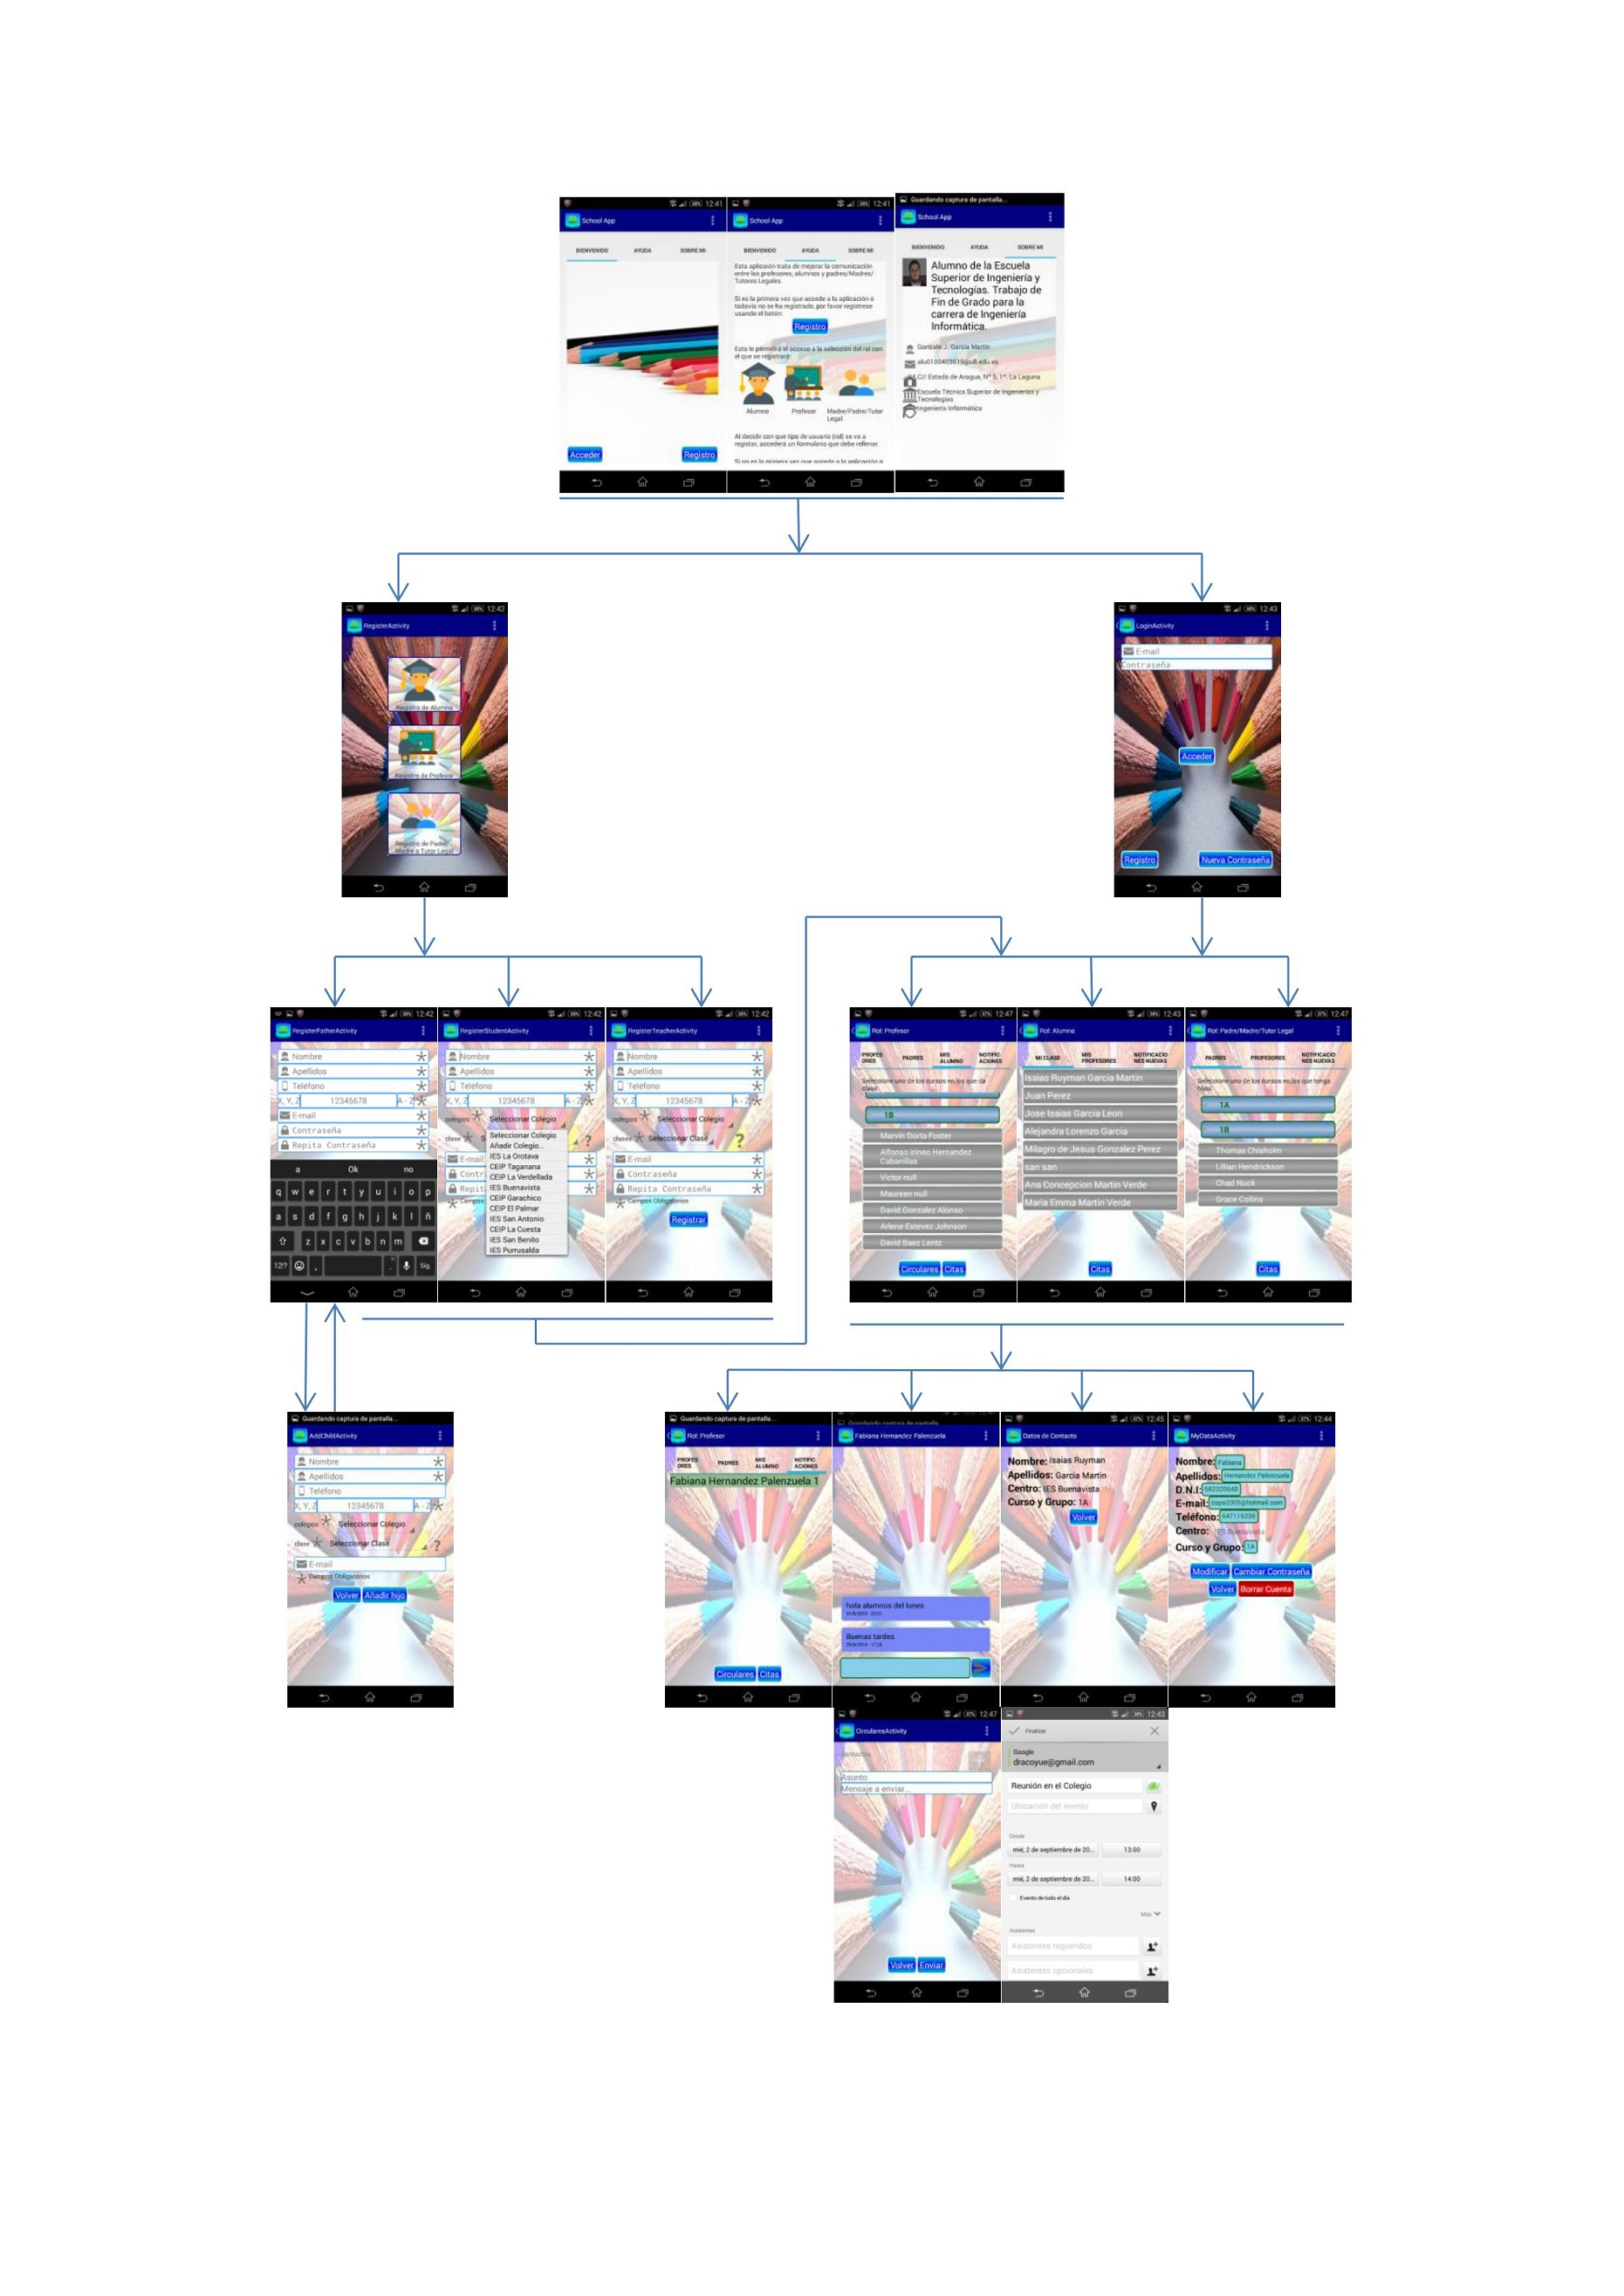
\includegraphics[scale=1.3]{mapaActividades}
		\caption{Navegación en las pantallas de \CollegeApp.}
		\label{fig:ActivitiesSecuence}
	\end{figure}
	
	\newpage
	\section{Pantalla Principal ({\ttfamily MainActivity})}
		Es la {\it activity} principal a la que accede el usuario cuando inicia la aplicación. Esta se compone de tres {\it fragments}.
		
		\subsection{Bienvenida ({\ttfamily WelcomeFragment})} \label{sec:welcome}
			La pantalla que le da la bienvenida al usuario. Como se puede ver en la figura \ref{fig:welcome}, contiene dos botones. Un botón que lleva a la pantalla de registro (ver sección \ref{sec:register}) y otro que lleva a la pantalla de acceso a la aplicación (ver sección \ref{sec:login}).
			
			\begin{figure}[h !]
				\centering
				
\includegraphics[scale=0.4]{Imagenes/App/welcome}
				\caption{Pantalla de Bienvenida de la Aplicación.}
				\label{fig:welcome}
			\end{figure}
		
		\subsection{Ayuda ({\ttfamily HelpFragment})}
			
			En la figura \ref{fig:help} se puede observar una ayuda orientada al uso de la aplicación. Los usuarios pueden consultar en esta pantalla la información básica sobre \CollegeApp. El usuario puede deslizar la pantalla para ver toda la información.
			
			\begin{figure}[h !]
				\centering
				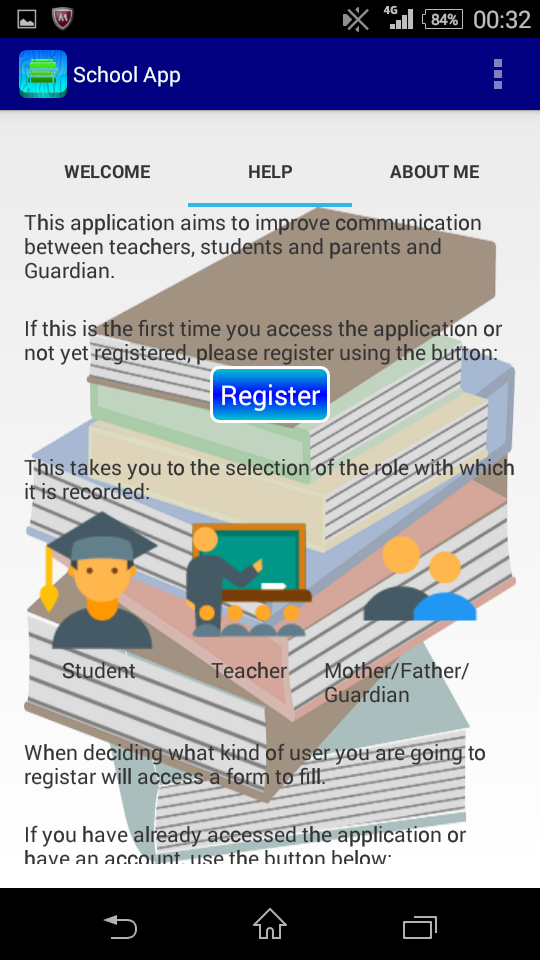
\includegraphics[scale=0.3]{Imagenes/App/help}
				\caption{Pantalla de ayuda de la Aplicación.}
				\label{fig:help}
			\end{figure}
		
		\subsection{Sobre mi ({\ttfamily AboutMeFragment})}
			En {\ttfamily AboutMeFragment} se encontrará la información referente al autor de la aplicación.
	
	\section{Cambio de idioma ({\ttfamily ChangeLanguajeActivity})}
	
		{\ttfamily ChangeLanguajeActivity} muestra los distintos idiomas disponibles de la aplicación. Al seleccionar uno de ellos y accionar el botón volver, quedará almacenado el idioma y las actividades lo cargarán al ser creadas. Los idiomas disponibles son español, inglés y francés, aunque con el mismo método se puede traducir la aplicación a cualquier otro idioma.
		Al seleccionar el idioma se cambia el lenguaje por defecto de la {\it máquina virtual de java} \cite{59:jvm:online} y al crear las actividades obtiene el texto de la aplicación en el idioma seleccionado.
			
	\section{Registro ({\ttfamily RegisterActivity})} \label{sec:register}
		
		En la actividad de registro se pueden observar los perfiles con los que se puede registrar un usuario. Al seleccionar cualquiera de los tres botones, mostrará la pantalla de registro correspondiente. Los usuarios se pueden registrar como alumno ({\ttfamily StudentRegisterActivity}), padre ({\ttfamily FatherRegisterActivity}) o profesor ({\ttfamily TeacherRegisterActivity}).
		
		\begin{figure}[h !]
			\centering
			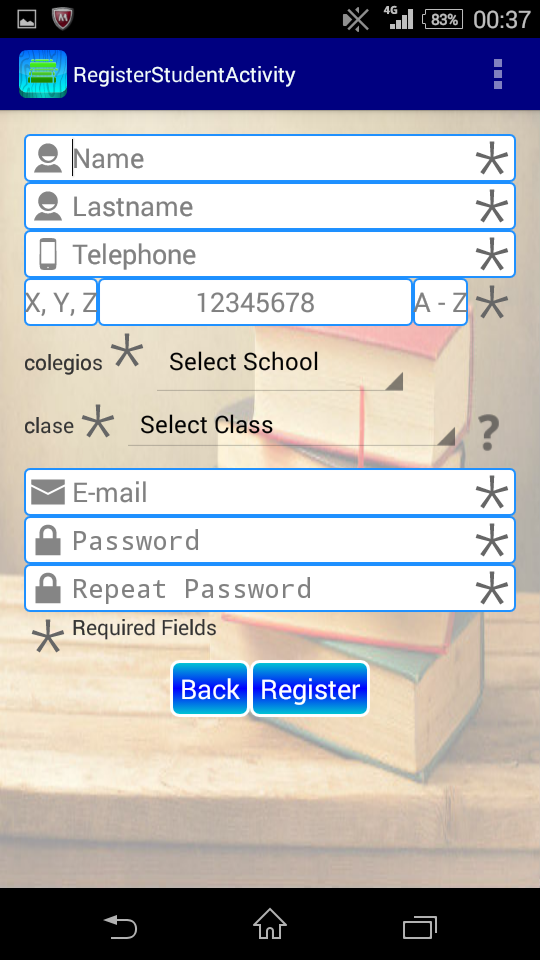
\includegraphics[scale=0.3]{Imagenes/App/registroAlumno}
			\caption{Pantalla de registro para el perfil de usuario.}
			\label{fig:StudentRegister}
		\end{figure}
		
		Las pantallas de registro (figura \ref{fig:StudentRegister}) muestran un formulario que el usuario deberá rellenar. Presentan dos botones, uno que le devolverá a la pantalla de bienvenida (sección \ref{sec:welcome}) y otro que completará el registro. La aplicación solo permitirá el registro si se han rellenado todos los campos obligatorios. Una vez hecho, al accionar el botón, la aplicación llevará a cabo el registro del usuario en la base de datos de {\it Firebase}. También se accederá de forma automática a la aplicación.
		
		\subsection{Añadir alumno ({\ttfamily AddChildActivity})} \label{sec:addChild}
			
			Si el usuario se registra como padre, debe registrar al menos a un alumno como hijo (figura \ref{fig:addChildRegister}). Al introducir los datos del estudiante, la aplicación consultará en la base de datos si existe el alumno. Si no existe se añadirá la información y se asociará con el padre, mientras que si existe solo se le asociará. Tras el registro del alumno volverá a mostrar la pantalla de registro de padres (sección \ref{sec:register}).
			
			\begin{figure}[h !]
				\centering
				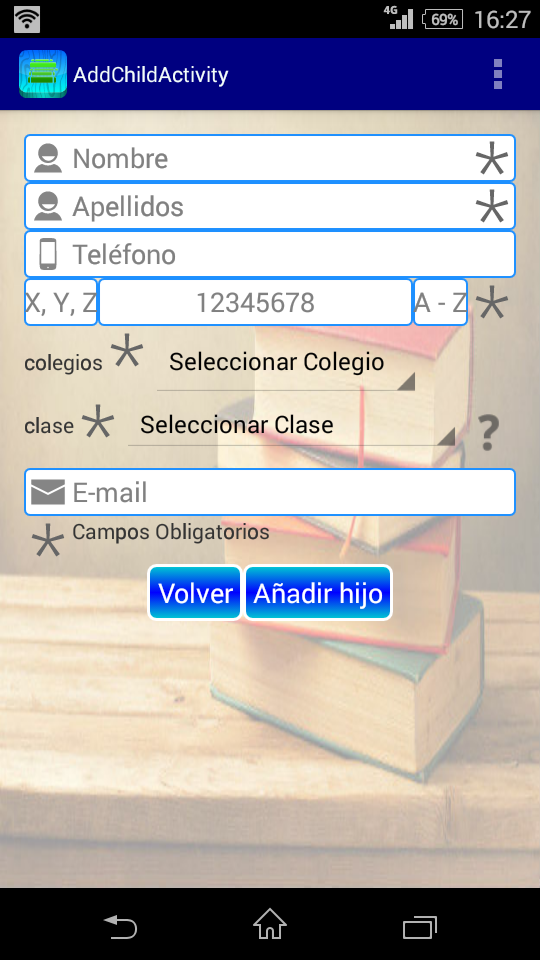
\includegraphics[scale=0.3]{Imagenes/App/addChild}
				\caption{Registro de hijos.}
				\label{fig:addChildRegister}
			\end{figure}
		
	\section{Acceso ({\ttfamily LoginActivity})} \label{sec:login}
		
		En {\ttfamily LoginActivity} (figura \ref{fig:loginLand}) se presentan dos campos en los que el usuario debe introducir su correo electrónico y contraseña para poder acceder a \CollegeApp\ con el botón de acceso. Si selecciona el de registro, se mostrará la pantalla de selección de perfil (Véase \ref{sec:register}). Para seleccionar {\it nueva contraseña} el usuario debe haber introducido previamente su correo electrónico. La aplicación se la solicitará al servidor de {\it Firebase} quien la enviará a la dirección con la que el usuario se ha registrado.
		
		\begin{figure}[h !]
			\centering
			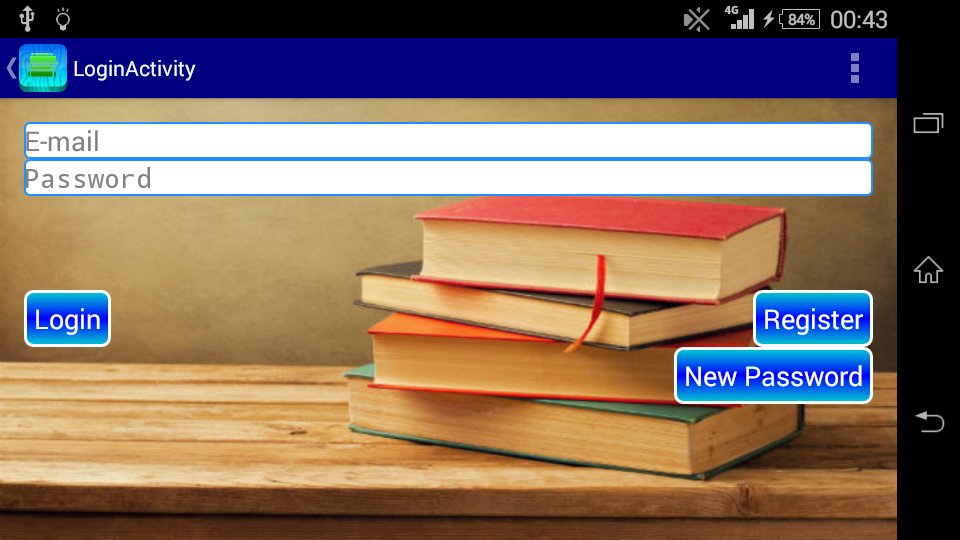
\includegraphics[scale=0.3]{Imagenes/App/loginLand}
			\caption{Pantalla de acceso con el dispositivo en horizontal.}
			\label{fig:loginLand}
		\end{figure}
	
	\section{Acceso de Usuarios}
	
		Al acceder a la aplicación, esta se encargará de consultar en la base de datos el rol del usuario. Si el acceso es correcto, se mostrará una pantalla con pestañas. Cada pestaña es una lista de contactos desplegable, excepto en el caso del alumno. También se mostrará una pestaña adicional para las notificaciones, es decir, mensajes que le lleguen al usuario (sección: \ref{sec:notifications}). En las opciones puede seleccionar cambiar sus datos (sección \ref{sec:myData}) y salir de la aplicación.
		Al seleccionar el botón citas (sección \ref{sec:dates}) se mostrará la pantalla encargada de añadir un evento al calendario del dispositivo. Esta funcionalidad viene implementada por el {\it sistema operativo}.
		
		\bigskip
		La figura \ref{fig:profeAlu} presenta un ejemplo del acceso de un usuario con el rol de profesor.
		
		\begin{figure}[h !]
			\centering
			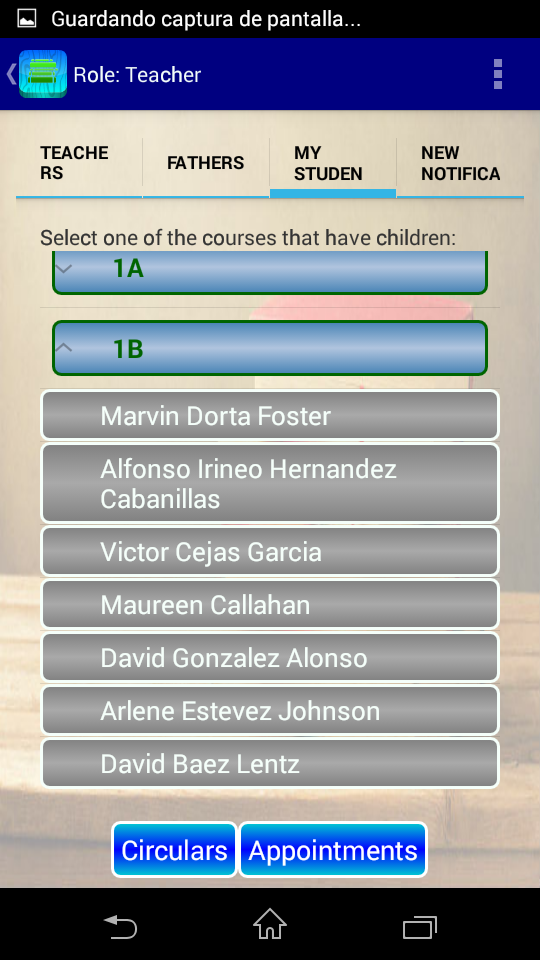
\includegraphics[scale=0.3]{Imagenes/App/profeAlu}
			\caption{Lista de contacto de alumnos para el perfil de profesor.}
			\label{fig:profeAlu}
		\end{figure}
	
	\section{Notificaciones ({\ttfamily notificationsActivity})} \label{sec:notifications}
	
		En la figura \ref{fig:notifications} se muestran todas las notificaciones que reciben los usuarios. Éstas son recuperadas y eliminadas de la base de datos en {\it Friebase}. La notificación muestra el nombre del remitente y el número de mensajes que ha enviado y que el usuario tiene sin leer. Se clasifican por colores según el perfil del usuario que las envía.
		Al seleccionar cualquiera de ellas se podrá comunicar de forma directa con mensajes tipo chat (sección \ref{sec:chat}) con el remitente.
	
		\begin{figure}[h !]
			\centering
			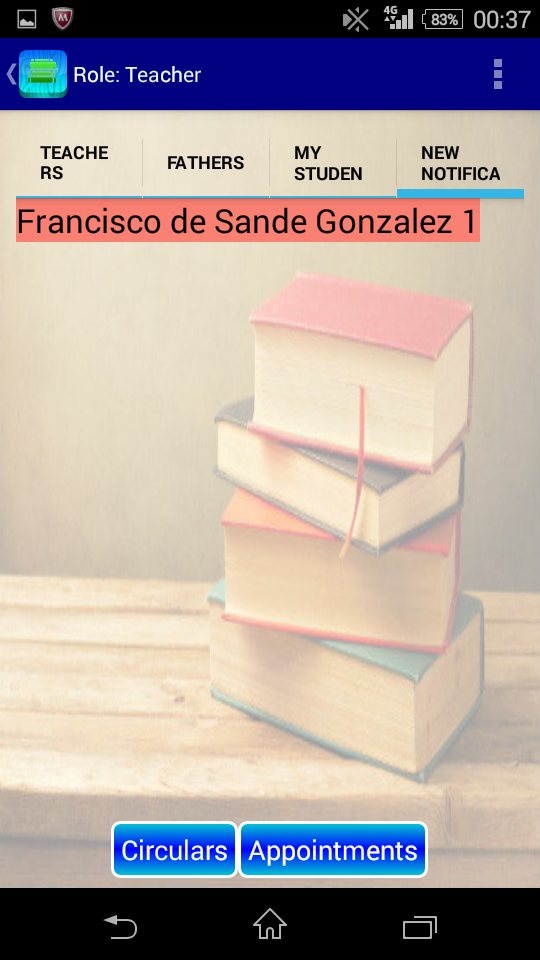
\includegraphics[scale=0.3]{Imagenes/App/Notifications}
			\caption{Notificaciones recibidas por los usuarios.}
			\label{fig:notifications}
		\end{figure}
	
	\section{Chat ({\ttfamily ChatActivity})} \label{sec:chat}
	
		En esta pantalla obtenemos mensajería directa tipo chat con cualquiera de los contactos del usuario. Estos mensajes se almacenan en la base de datos de {\it Firebase} de donde son recuperados y eliminados. También se guardan en una base de datos local, almacenada en el dispositivo. Si accedemos a las opciones podemos eliminar la conversación.
	
	\section{Mis Datos ({\ttfamily MyDataActivity})} \label{sec:myData}
	
		En la figura \ref{fig:myData} se puede observar que el usuario puede ver los datos con los que se registró. Al seleccionar el botón modificar, podrá cambiar sus datos salvo el D.N.I. y el correo electrónico. Como un usuario conservará el mismo número en el documento nacional de identidad durante toda su vida, no se contempla que se pueda modificar. Con respecto al correo electrónico, es la clave con que el usuario se autentica contra el servidor, por lo cual no se podrá modificar para evitar inconsistencia de datos.
		
		\bigskip
		Si selecciona guardar se modificará la base de datos en el proveedor de servicios.
		Si selecciona dar de baja su cuenta, se borrará la información que hay en {\it Firebase}. También puede cambiar su contraseña con el botón destinado a ello (sección \ref{sec:changePassword}).
		
		\begin{figure}[h !]
			\centering
			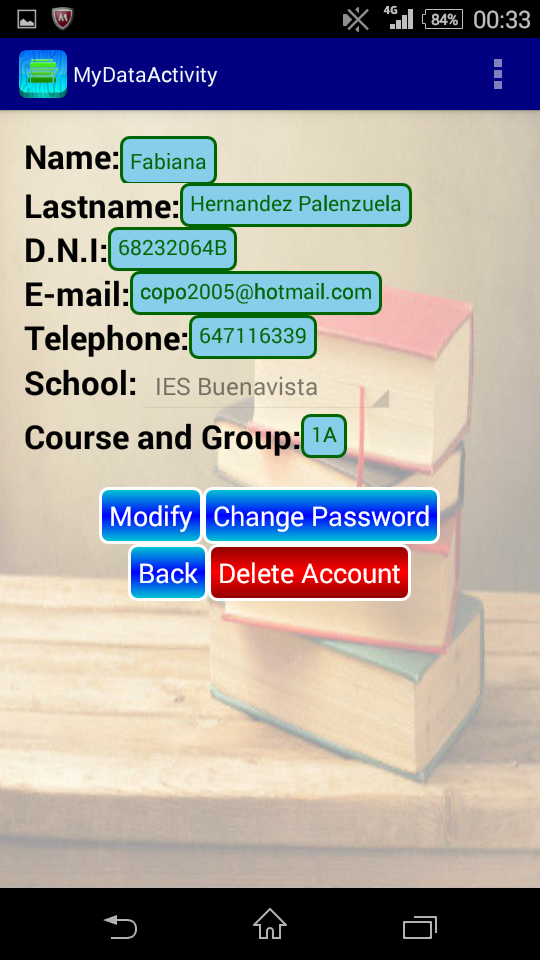
\includegraphics[scale=0.3]{Imagenes/App/myData}
			\caption{Datos del usuario.}
			\label{fig:myData}
		\end{figure}
	
	\section{Cambio de Contraseña ({\ttfamily ChangePasswordactivity})} \label{sec:changePassword}
	
		En la pantalla de cambio de contraseña el usuario podrá cambiar su contraseña introduciendo su correo electrónico y contraseña antigua. También deberá seleccionar una nueva contraseña y repetirla. Si desea hacer el cambio permanente solo deberá accionar el botón guardar.
	
	\section{Circulares ({\ttfamily CircularesActivity})} \label{sec:circulares}
	
		En {\ttfamily CircularesActivity} se podrá enviar un mismo mensaje a una o varias clases, ya sean alumnos o padres. Al seleccionar el botón enviar, se enviará el mismo mensaje a cada uno de los alumnos que pertenezca a la clase seleccionada.
	
	\section{Citas} \label{sec:dates}
		Esta funcionalidad usa el calendario del dispositivo. Lanza la actividad que permite añadir eventos. Viene implementado en el {\it sistema operativo}.
		Se introducen los datos en los campos correspondientes y luego se selecciona guardar. Se puede elegir el calendario en el que almacenar el evento, en el dispositivo o en el de {\it Google}.
	
	\section{Datos del contacto ({\ttfamily DataActivity})} \label{sec:data}
	
		En {\ttfamily DataActivity} se muestran los datos de cualquier contacto del usuario.